\documentclass[tikz,border=8pt]{standalone}
\usepackage{amsmath}
\usetikzlibrary{arrows.meta}
\definecolor{ink}{HTML}{21352F}\definecolor{teal}{HTML}{087F7B}
\definecolor{blue}{HTML}{4B77A8}\definecolor{gold}{HTML}{C58B2A}
\begin{document}
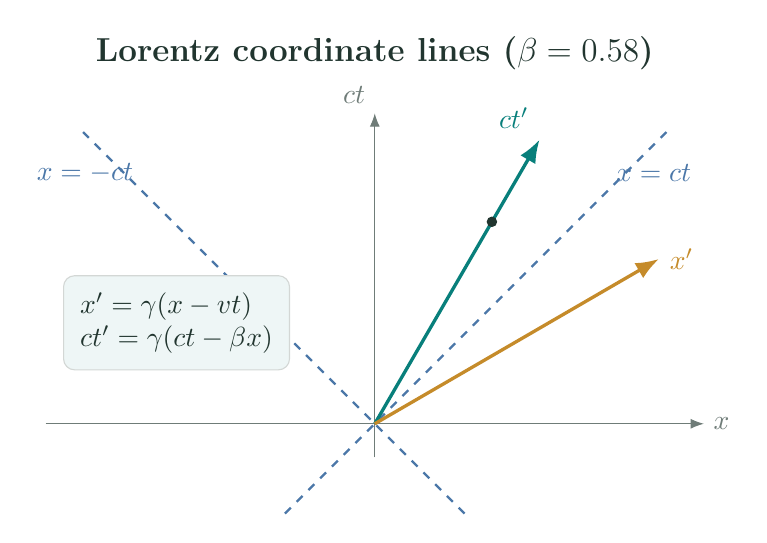
\begin{tikzpicture}[font=\sffamily,text=ink,>=Latex,scale=.95]
  \def\bet{0.58}
  \node[font=\bfseries\large] at (0,4.95) {Lorentz coordinate lines ($\beta=0.58$)};
  \draw[->,ink!65] (-4.4,0)--(4.4,0) node[right] {$x$};
  \draw[->,ink!65] (0,-.45)--(0,4.15) node[above left] {$ct$};
  \draw[blue,thick,dashed] (-1.2,-1.2)--(3.9,3.9);
  \draw[blue,thick,dashed] (1.2,-1.2)--(-3.9,3.9);
  \node[blue,anchor=west] at (3.1,3.35) {$x=ct$};
  \node[blue,anchor=east] at (-3.1,3.35) {$x=-ct$};
  \draw[teal,very thick,->] (0,0)--({\bet*3.8},3.8) node[above left] {$ct'$};
  \draw[gold,very thick,->] (0,0)--(3.8,{\bet*3.8}) node[right] {$x'$};
  \fill[ink] ({\bet*2.7},2.7) circle (2pt);
  \node[align=left,draw=ink!20,fill=teal!7,rounded corners=4pt,inner sep=6pt] at (-2.65,1.35)
    {$x'=\gamma(x-vt)$\\$ct'=\gamma(ct-\beta x)$};
\end{tikzpicture}
\end{document}
